% ------------------------------------------------
% Page start
% ------------------------------------------------
\chapter{Introduction}
\label{chap:introduction}

\baselineskip=26pt
\thispagestyle{empty}
% ------------------------------------------------

Because of the grow of cloud computation, we are already in the era of data deluge that the data grow rapidly which can produced multiple petabyte per day. The problem no longer is the out of disk capacity, but the data is outgrowing the capabilities of the searching process that can't return the result instantly in the modern relational database. But the data will still grow continually, so the respond time will become longer and longer. For example if wish to mining ten petabyte data, it can take few days or week, this is not fast enough for some application such as the use of the government or science research. So how to solve this kind of problem become a most significant subject \cite{paper:nodb}.\\

To lower the searching time of the database, more and more people started using the non-relational database from relational database to seek less respond time. But this may meet some problem such as most non-relational database are using as key-value, so if you want to retrieve a value, you need to know its key, but you can't using the value to find the key or using conditional searching (like the 'WHERE Clause' in SQL) to search the key or value, also normally non-relational database can't use SQL as query language. This will cause some feature which basic on the query operation un-functional in program, this may need to modify tons of code to become useable. So if the program architecture don't need highly relational, more and more that kind of application swap using the non-relational database from relational database (In the blog of Planet Cassandra, they sometimes posts a new about some company swapping their database from relational database to Cassandra \cite{web:planetcassandra-blog}).\\

Non-relational database是使用DHT (distributed hash table) \cite{web:wiki:distributed_hash_table}的架構, 所以searching能在O(1)的時間完成, 比relational database的已做indexing的O(log(n))或full table scan的O(n)來得快很多, 尤其是發生在relational database的row很巨量的時候, 不管是在search, delete還是join (尤其在table巨大時, join會需要大量的處理時間和memory空間) 上.\\

因為non-relational database是使用hash table的key-value方式來stores, 故data store是不須以relational database的table模式來存放, 但如果想使原本table設計的話, 可使用把row的多個column變成多個key, 就能馬上得到同樣table的效果.\\

Therefore, non-relational database is a very advantage thing, but it lack some feature which exist in relational database (query, join operation, indexing, comparison, etc. ).\\

Normal searching a key from value in non-relational database which can be done in three ways: range scan, full scan or MapReduce.\\

First full scan takes huge of times, second the range scan can't target on value, even the programmer know the range of the data, it still may cost times if there is many keys but the value is not wanted or it is can't found the result which have different length of the key in the same query. This kind of problem increase the work load to the programmer, which will slow down the whole process which the programmer working.\\

So the best way seem to be using the MapReduce \cite{paper:google-mapreduce,web:wiki:mapreduce} to distribute all keys to many server and search it to find the result.\\

\begin{figure}[h]
\centering
%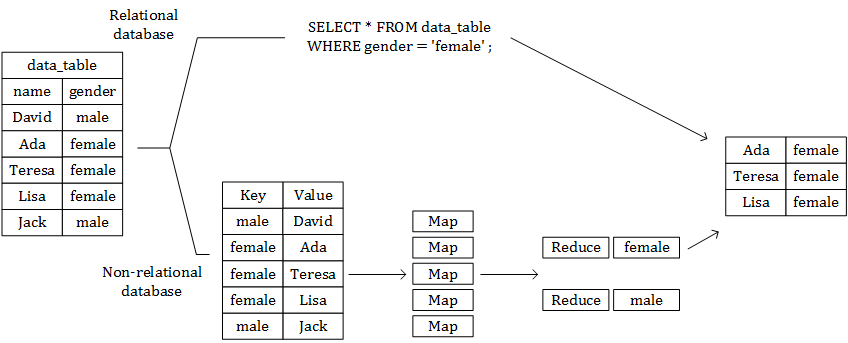
\includegraphics[scale=0.6]{./introduction/pic/mapreduce_v3.png}
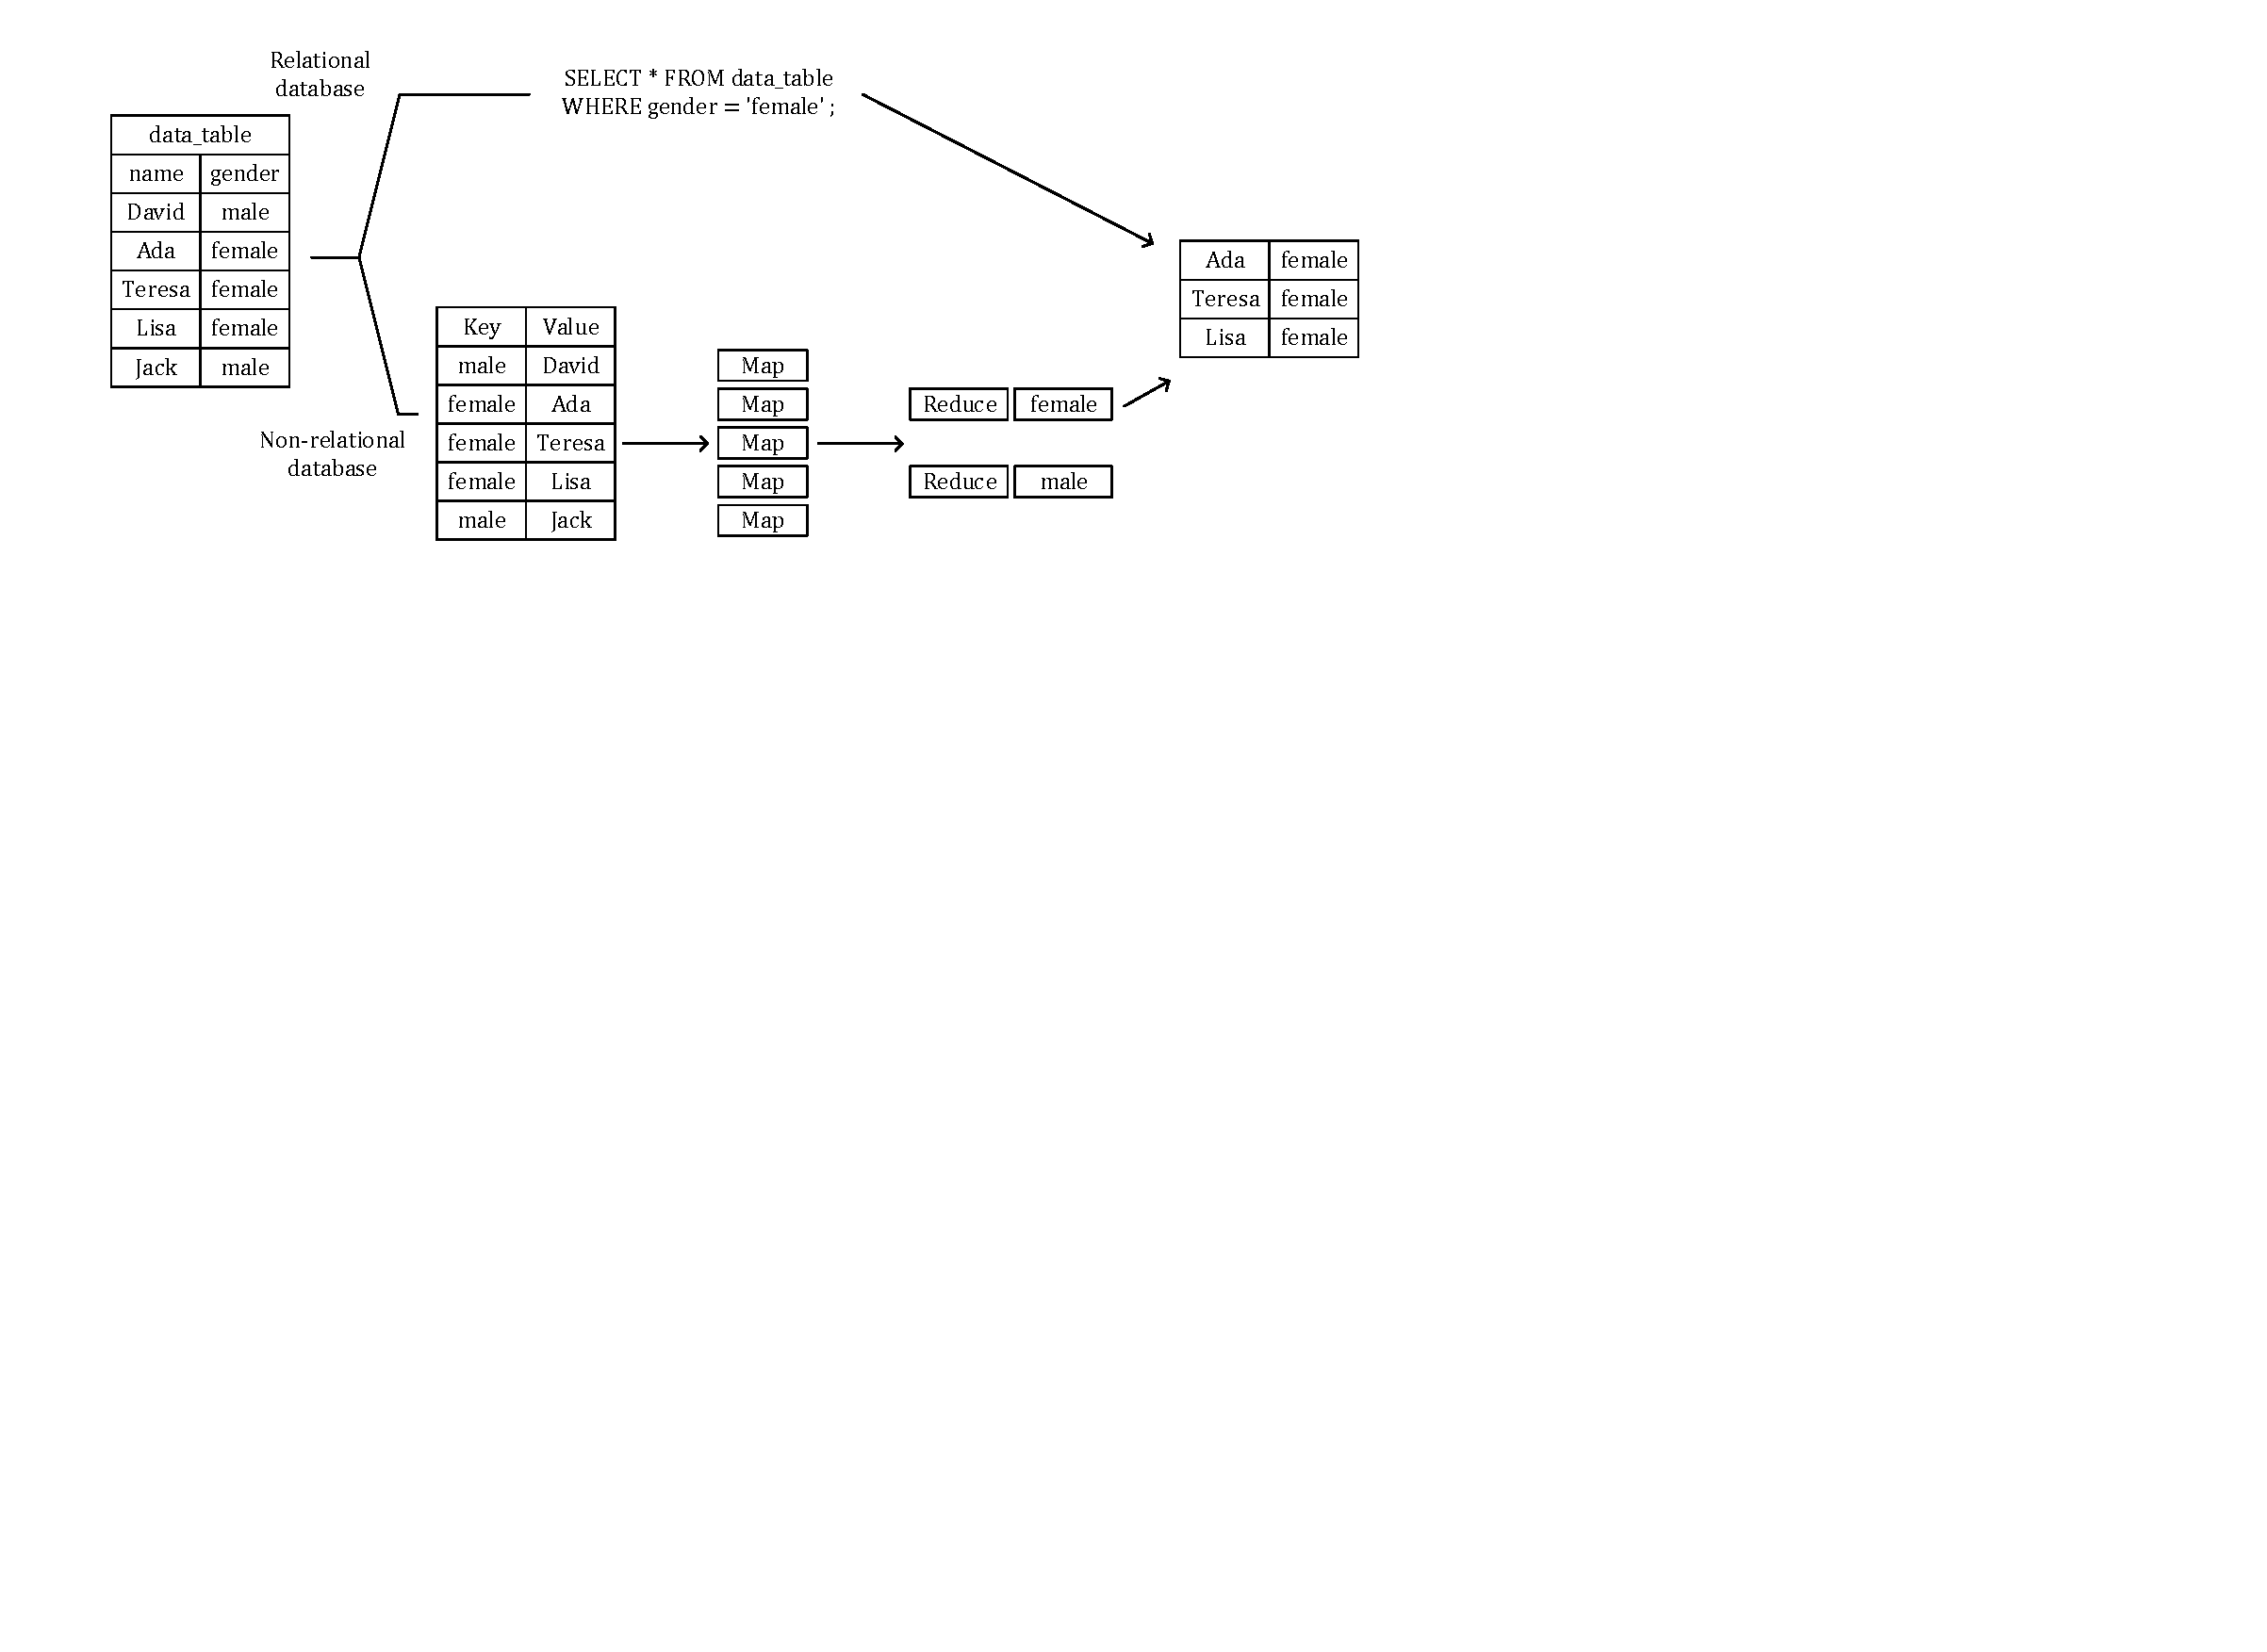
\includegraphics[width=0.9\textwidth]{./introduction/pic/mapreduce_v3.pdf}
\caption{A example of using MapReduce for searching key from value.}
\label{fig:intro:mapreduce}
\end{figure}

Figure \ref{fig:intro:mapreduce} is an example that there is some data about the people, and we want to find out the people who is female. It is very easy for relational database by using the SQL, but it is difficult to non-relational database. Which normally using the unique data as the key which is the gender as this case, then the name will become the value to use MapReduce.\\

But if using the MapReduce that have some disadvantages such as:

\begin{enumerate}

\item Programmer need to learn how to write MapReduce program.

\item No all non-relational database provide MapReduce, so some of it need to combine with Hadoop to make it work, this increase the difficult for architecture designer.

\item When assigning the jobs for MapReduce, the JobTracker in master node need to store all the job's metadata, so if using key-value pair to create mapping and created a large number (such as same number of keys, for example one million keys) of mapping, this will need a huge number of memory which means the hardware still need some requirement.

\item The time of assigning the jobs and waiting its complete is slow. If the program always need to do this kind of searching, the performance will become very low.

\end{enumerate}

So using MapReduce is a workable way but it has its own limit.\\

Formerly if the data size is not big enough (like dozens gigabytes), it can wait few more second or minute for the result. But if the data become multiple petabyte, if still using the same thought which will become few more hours or days, it could be months worst, that is unacceptable in many application which need to response instant. So some people using the cluster concept to distribute the work to decrease the work time per machine. But actually using a suitable indexing method by using the storage to reduce time, it can be found the result in few second on multiple petabyte data, and the machine don't need to be a high-level machine, and this is the core concept of this paper.\\

This paper is to propose the Li's Hash --- an indexing algorithm for key-value stores. By adding indexing feature to key-value store, then it can have the query feature as the relational database did, also it can search to result on single machine rather than using MapReduce.\\

Li's Hash is an algorithm that combines the concept of n-gram indexing \cite{web:wiki:n-gram} (Figure \ref{fig:intro:n-gram}), JSON (JavaScript Object Notation) \cite{web:wiki:json} (Figure \ref{fig:intro:json_example}) and hash table \cite{web:wiki:hash-table}.\\

JSON is exactly as same as hash table but it can store different data type of data, not just one data type only.

\begin{figure}[h]
\centering
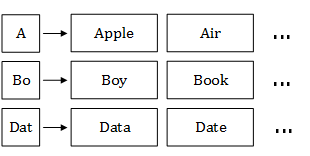
\includegraphics[scale=0.6]{./introduction/pic/n-gram_v1.png}
\caption{A example of n-gram indexing.}
\label{fig:intro:n-gram}
\end{figure}

\begin{figure}[h]
\centering
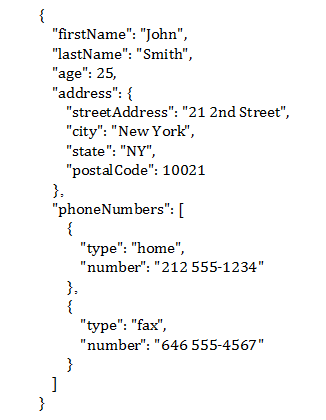
\includegraphics[scale=0.6]{./introduction/pic/json_example_v1.png}
\caption{A example of JSON.}
\label{fig:intro:json_example}
\end{figure}

And the n-gram indexing normally only target the data in string. But combining all of them can become a special structure which can store the data and query different data type of data, this can very useful for all kind of query and storage system design.\\

Li's Hash considered how the write the index data to disk, but if design is not good enough that will meet many problem such as I/O, synchronous, performance, etc. that the problem which is common to a database design. So we decided using modularized design for swappable the back-end database (The back-end can be an embedded database or the client side of a database server) for the user needed, this makes Li's Hash more flexibility and can focus on the algorithm design.\\

We have implemented a prototype to provide as a library \cite{web:lishash:home-page} that the user can use relational or non-relational APIs with different back-end non-relational database, just only need to modify the code for connecting to our library, then they don't need to modified any schema in original design, and keep the relational database concept to use non-relational database without need to learn any new concept about the back-end database.\\

\clearpage

% ------------------------------------------------
% End of page
% ------------------------------------------------
